\documentclass[12pt]{article}
\usepackage[utf8]{inputenc}
\usepackage[T1]{fontenc}
\usepackage{graphicx}
\usepackage{xcolor}
\usepackage[linewidth=1pt]{mdframed}
\usepackage{xeCJK}

%%novalidate

\usepackage{tikz}
\usepackage{calc}
\usepackage{booktabs}


% colors
\definecolor{color1}{HTML}{000060}
%\definecolor{color1}{HTML}{8C260F}
\definecolor{color2}{HTML}{333333}


% fonts
\usepackage{fontspec}
\defaultfontfeatures{Mapping=tex-text}
\setmainfont
[BoldFont=Lato-Bold.ttf,
ItalicFont=Lato-Italic.ttf,
BoldItalicFont=Lato-BoldItalic.ttf]
{Lato-Regular.ttf}
\newfontfamily\headingfont[ItalicFont=Lato-BlackItalic.ttf]{Lato-Black.ttf}
%%%

\usepackage{geometry}
\geometry{a4paper,
hmargin=20mm,vmargin=20mm,
head=0ex,foot=3ex}

\linespread{1.3}

\usepackage[hang]{caption}
\DeclareCaptionFormat{upper}{#1#2\uppercase{#3}\par}
\captionsetup{labelfont={bf,color=color2},textfont={normalsize,color=color2},format = upper,figurename=FIGURE,tablename=TABLE}

%%% fancy sections
\usepackage{titlesec}
%\titleformat{\chapter}{\headingfont\LARGE\bfseries\scshape\color{color1}}{\thechapter}{1em}{}[\titlerule]
\titleformat{\section}{\color{color1}\headingfont\Large\bfseries\uppercase}{\thesection}{1em}{}[\titlerule]
\titleformat{\subsection}{\color{color1}\headingfont\large\bfseries\uppercase}{\thesubsection}{1em}{}
\titleformat{\subsubsection}{\color{color1}\headingfont\bfseries\uppercase}{\thesubsubsection}{1em}{}
%%%

% head and foot
\usepackage{fancyhdr}
\pagestyle{fancy}
\lhead{}
\chead{}
\makeatletter
\rhead{\color{color2}\@date}
\makeatother
\newlength{\myheight}
\lfoot{
\settoheight{\myheight}{\thepage}
\raisebox{-2ex-0.5\myheight}{
\includegraphics[height=4ex]{logo}}
}
\cfoot{\color{color2}\LaTeX\ template for business reports}
\rfoot{\color{color2}\thepage}
\renewcommand\headrulewidth{0pt}
\renewcommand\footrulewidth{0pt}

% custom titlepage
\makeatletter
\newcommand*\DefVar[1]{\@namedef{#1}##1{\global\@namedef{get#1}{##1}}}
\DefVar{summary}
\renewcommand{\maketitle}{
\begin{center}

\begin{tikzpicture}
    \node[draw=none,%color1,line width=0.4pt,
      fill=color1,
      inner sep = 10pt,
      text width=\textwidth-20pt,
      text centered
    ] {\color{white}\headingfont\bfseries\huge\@title};
\end{tikzpicture}
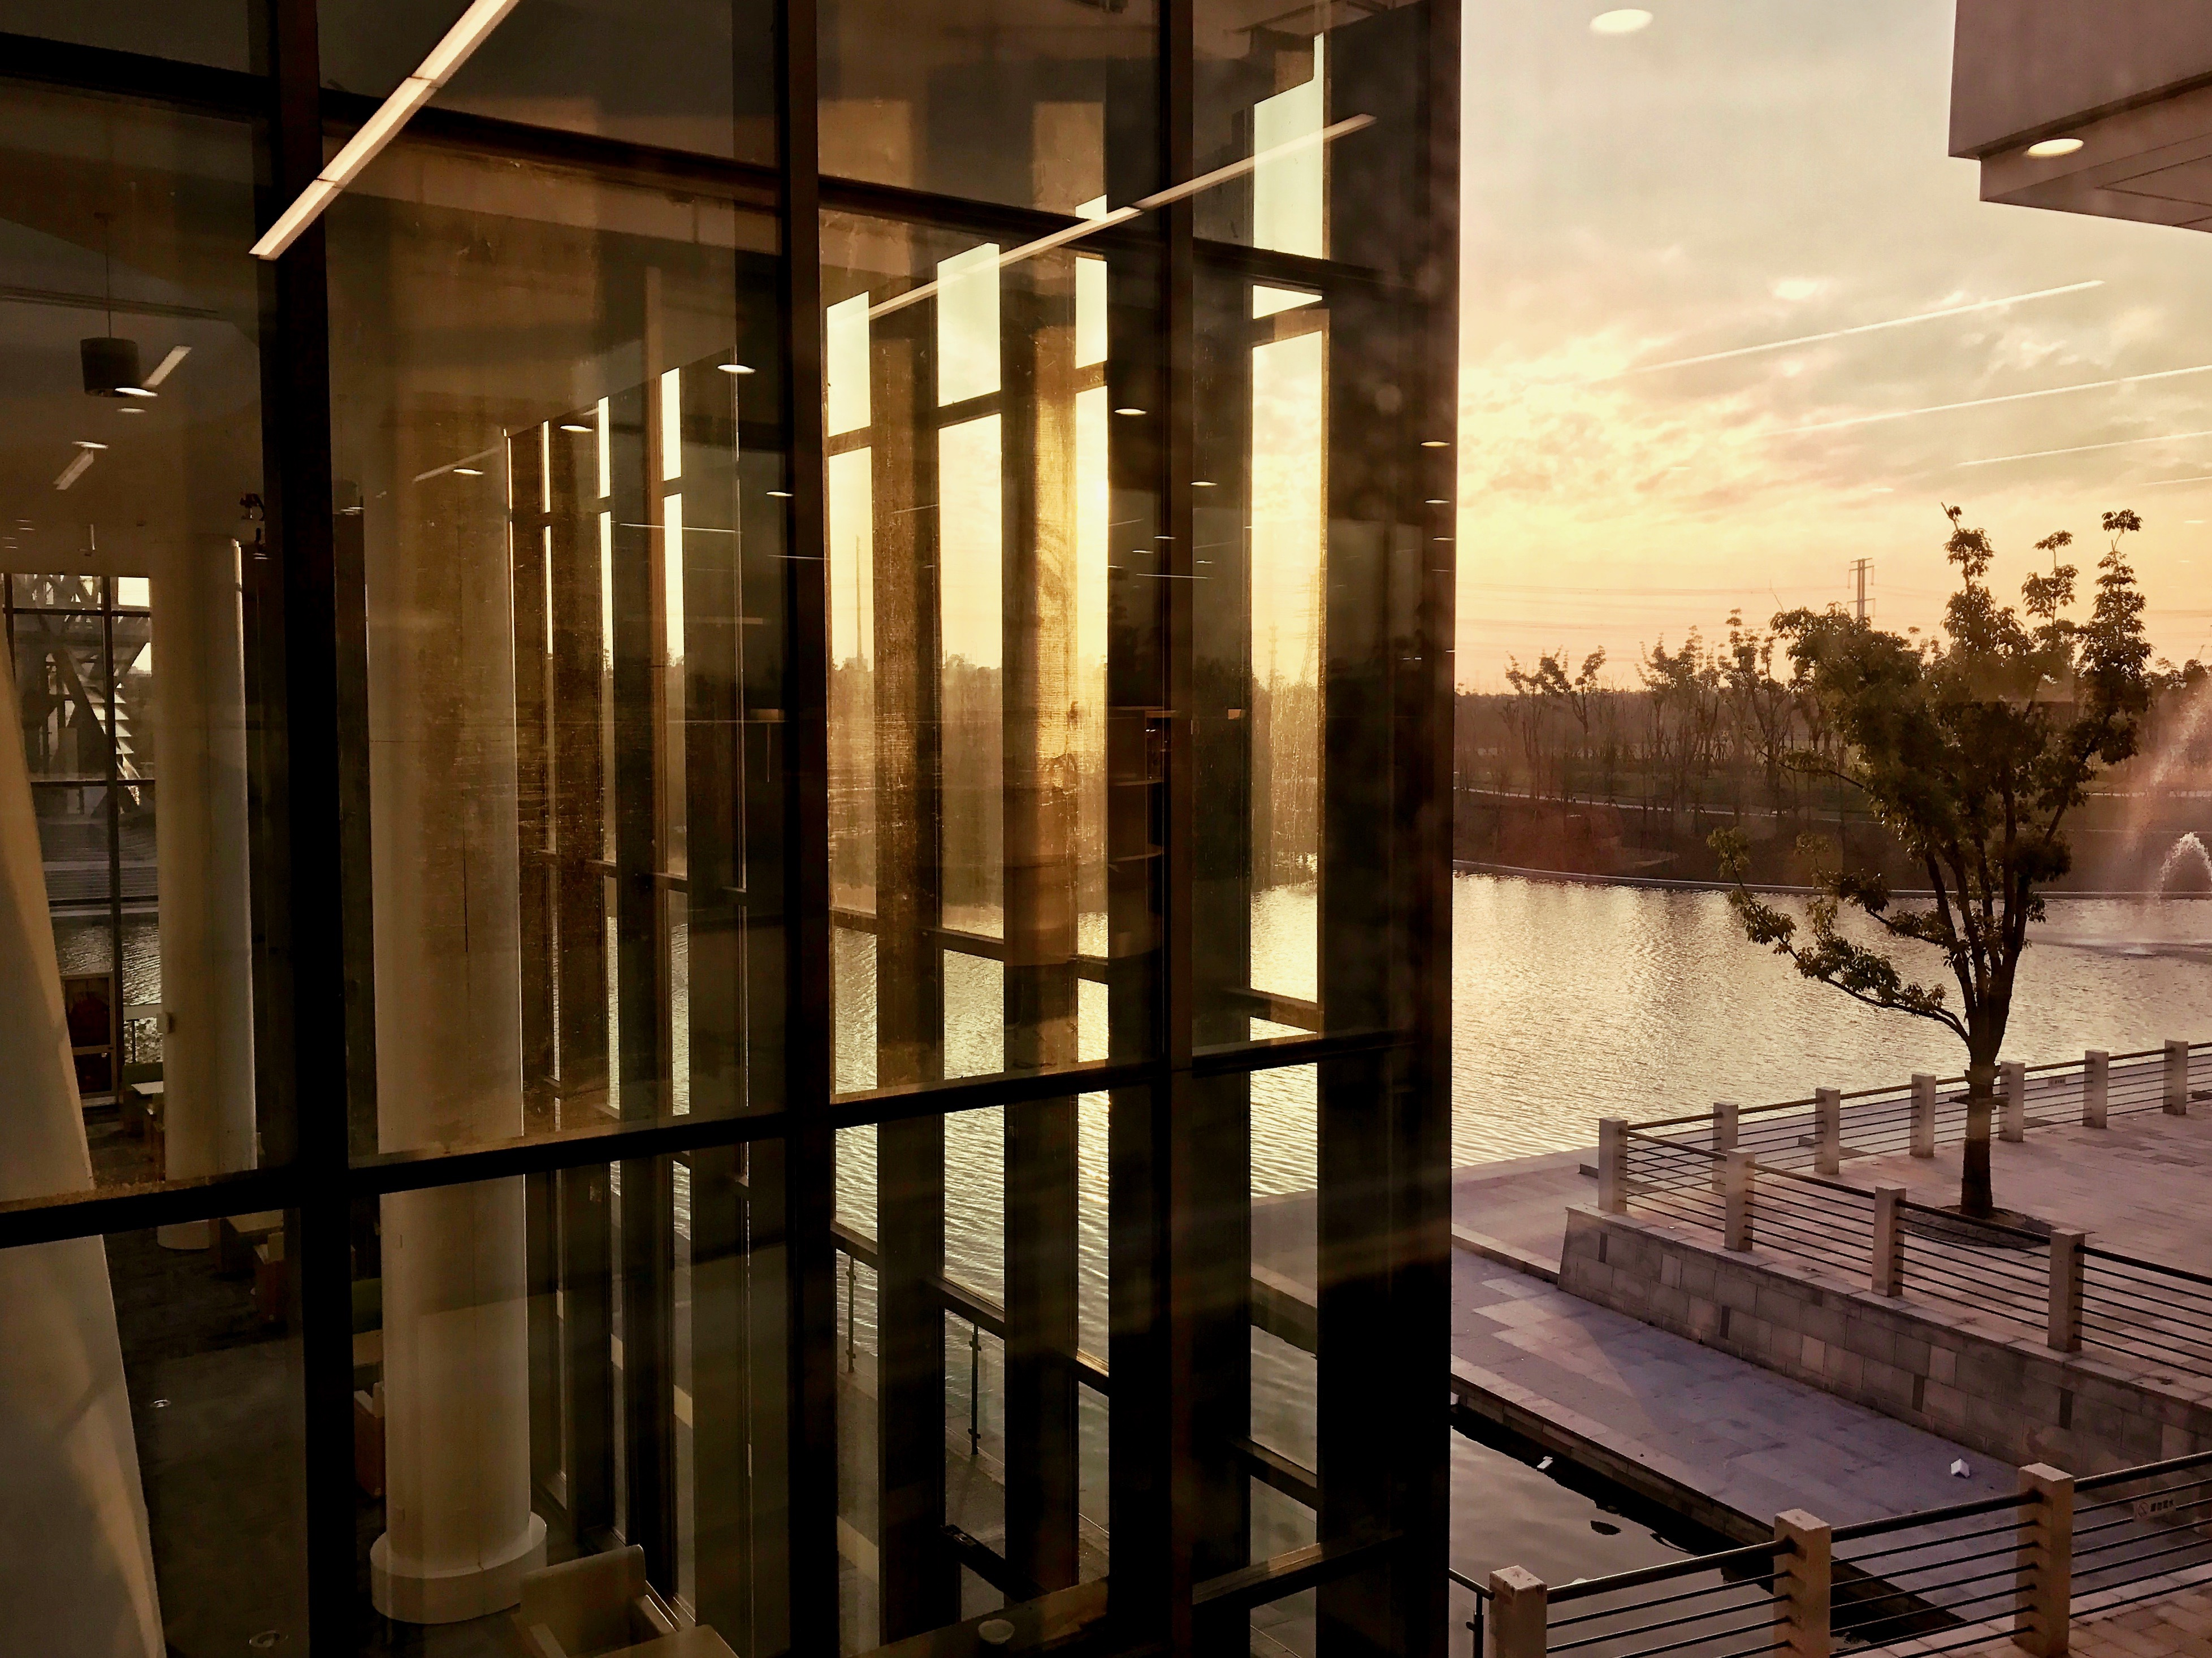
\includegraphics[width=\textwidth]{opening}\par
\headingfont\bfseries\Large\@author\par
\bigskip\medskip
{\color{color2}\normalfont\normalsize\textbf{Summary:}\\
\getsummary}
\end{center}
\clearpage
}
\makeatother
%%%

%%% fancy boxes
\usepackage{tcolorbox}
\usepackage{wrapfig}
\def\fullboxbegin{
\bigskip
\begin{tcolorbox}[colback=color1,colframe=color1,coltext=white,arc=0mm,boxrule=0pt]
}
\def\fullboxend{\end{tcolorbox}\medskip}
%
\def\leftboxbegin{
\begin{wrapfigure}{l}{0.5\textwidth}
\begin{tcolorbox}[colback=color1,colframe=color1,coltext=white,arc=0mm,boxrule=0pt]
}
\def\leftboxend{
\end{tcolorbox}
\end{wrapfigure}
}
%
\def\rightboxbegin{
\begin{wrapfigure}{r}{0.5\textwidth}
\begin{tcolorbox}[colback=color1,colframe=color1,coltext=white,arc=0mm,boxrule=0pt]
}
\def\rightboxend{
\end{tcolorbox}
\end{wrapfigure}
}
%
\newcounter{frames}
\def\frameboxbegin#1{
\bigskip
\refstepcounter{frames}
\begin{tcolorbox}[colback=white,colframe=color1,arc=0mm,title={\MakeUppercase{\textbf{Frame \arabic{frames}}: #1}}]
}
\def\frameboxend{
\end{tcolorbox}
}
%%%

\usepackage{lipsum}


\usepackage{tikz,mathpazo}
\usetikzlibrary{shapes.geometric, arrows}
\usetikzlibrary{calc}


\title{Digital Clock - JEHHEJ}
\author{JEHHEJ\\ Huangyq /Hongry }
\date{\today}
\summary{ A LED digital clock
}


\begin{document}
\maketitle

\tableofcontents
\clearpage

\section{Introduction}

\section{Workflow}

\includegraphics[scale=0.75]{workflow}

\section{Components}
\begin{table}[!h]
\centering
\caption{Component List.}
\begin{tabular}{ccc}
\toprule
Name & Type  & Quantity \\
\midrule
 Battery Box  &    & 1  \\
 Timer555 &   & 1 \\
 Capactior  & 0.01$\mu$F   & 1  \\
     & 0.1$\mu$F  & 1 \\
Resistor & 1k$\Omega$  & 1 \\
     &  2k$\Omega$ & 1 \\
     &  100$\Omega$ & 3 \\
JK Flip Flop   & 74HC112  & 27 \\
Seven Seg Display  &    & 12  \\
Seven Seg Encoder&  74LS48D  & 12  \\
Switch  &    & 10  \\
NOT Gate  & 74AS04M & 20  \\
NAND Gate  & 7400N & 20  \\
XOR Gate  & 7486N & 10  \\
OR Gate  & 7432N & 5  \\
Piezo Buzzer & & 1  \\
CMOS & IRF510 & 4  \\
LED & White & 10  \\

\bottomrule
\end{tabular}
\end{table}

\clearpage
\section{Circuit Principle}

\section{Block Schematic}

\thispagestyle{empty}
\tikzstyle{startstop} = [rectangle, rounded corners, minimum width=3cm, minimum height=1cm,text centered, draw=black, fill=red!30]
\tikzstyle{io} = [trapezium, trapezium left angle=70, trapezium right angle=110, minimum width=1cm, minimum height=0.8cm, text centered, draw=black, fill=orange!30]
\tikzstyle{process1} = [rectangle, minimum width=3cm, minimum height=1cm, text centered, text width=3cm, draw=black, fill=yellow!30]
\tikzstyle{process2} = [rectangle, minimum width=3cm, minimum height=1cm, text centered, text width=3cm, draw=black, fill=blue!30]
\tikzstyle{process3} = [rectangle, minimum width=3cm, minimum height=1cm, text centered, text width=3cm, draw=black, fill=brown!30]
\tikzstyle{process4} = [rectangle, minimum width=3cm, minimum height=1cm, text centered, text width=3cm, draw=black, fill=green!30]
\tikzstyle{decision} = [diamond, minimum width=3cm, minimum height=1cm, text centered, draw=black, fill=green!30]
\tikzstyle{arrow} = [thick,->,>=stealth]

\begin{tikzpicture}[node distance=2cm]
\node (start) [startstop] {Power Supply 6V};
\node (in) [startstop, above of=start, yshift=0.5cm, xshift=2cm, yshift=1cm] {Function generator};
\node (pro1_1) [process1, right of=start, xshift=2cm] {Turn On/Off Time Ajustment Part};
\node (pro1_2) [process1, right of=pro1_1, xshift=2cm] {Reset Ajustment};
\node (pro2_1) [process2, above of=pro1_1, yshift=0.5cm,xshift=2cm] {Counter};
\node (pro2_2) [process2, above of=pro2_1] {Encoder};
\node (pro2_3) [process2, above of=pro2_2] {Seven Seg Display};
\node (pro3_1) [process3, right of=pro2_1, xshift=2cm] {DIY Encoder};
\node (pro3_2) [process3, right of=pro3_1, xshift=2cm] {7 LEDs\\(to represent for days from Mon. to Sun.)};
\node (pro4_1) [process4, below of=pro1_1, yshift=-0.7cm] {Set OR Part};
\node (pro4_2) [process4, right of=pro4_1, xshift=2cm] {Comparison Part};
\node (pro4_3) [process4, below of=pro4_1] {Turn On\&Off Alarm Part};
\node (pro4_4) [process4, right of=pro4_3, xshift=2cm] {Setting Part Via Counter};
\node (pro4_5) [process4, below of=pro4_4] {Encoder};
\node (pro4_6) [process4, below of=pro4_5] {7 Seg Display};
\node (pro4_7) [process4, right of=pro4_2, xshift=2cm] {7 Seg Display};

\draw [arrow](start) -- (pro1_1);
\draw [arrow](start) |- (pro2_1);
\draw [arrow](start) |- (pro2_2);
\draw [arrow](start) -- (0,1.5) -| (pro3_1);
\draw [arrow](start) -- (0,-5.9)-- (7,-5.9)--(7,-5.3);
\draw [arrow](start) -- (0,-1.5) -| (pro4_2);
\draw [arrow](pro2_1) -- (6,-2.7);
\draw [arrow](pro1_2) -- (pro2_1);
\draw [arrow](in) -- (pro2_1);
\draw [arrow](pro2_1) -- (pro3_1);
\draw [arrow](pro3_1) -- (pro3_2);
\draw [arrow](pro1_1) -- (pro1_2);
\draw [arrow](pro2_1) -- (pro2_2);
\draw [arrow](pro2_2) -- (pro2_3);
\draw [arrow](start) |- (pro4_1);
\draw [arrow](start) |- (pro4_5);
\draw [arrow](pro1_1) -- (pro1_2);
\draw [arrow](pro1_1) -- (in);
\draw [arrow](pro4_1) -- (pro4_2);
\draw [arrow](pro4_2) -- (pro4_7);
\draw [arrow](pro4_3) -- (pro4_1);
\draw [arrow](pro4_3) -- (pro4_4);
\draw [arrow](pro4_4) -- (pro4_5);
\draw [arrow](pro4_5) -- (pro4_6);

\end{tikzpicture}
\frameboxbegin{Color Block}
Red Block: Input\\
Purple Block: Basic Digital Clock\\
Yellow Block: Time Adjust Part\\
Brown Block: Show-Day Part\\
Green Block: Alarm Part
\frameboxend
\clearpage

\subsection{Input}
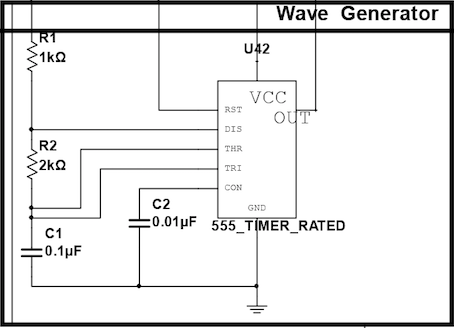
\includegraphics{Input.png}

\subsection{Basic Digital Clock}
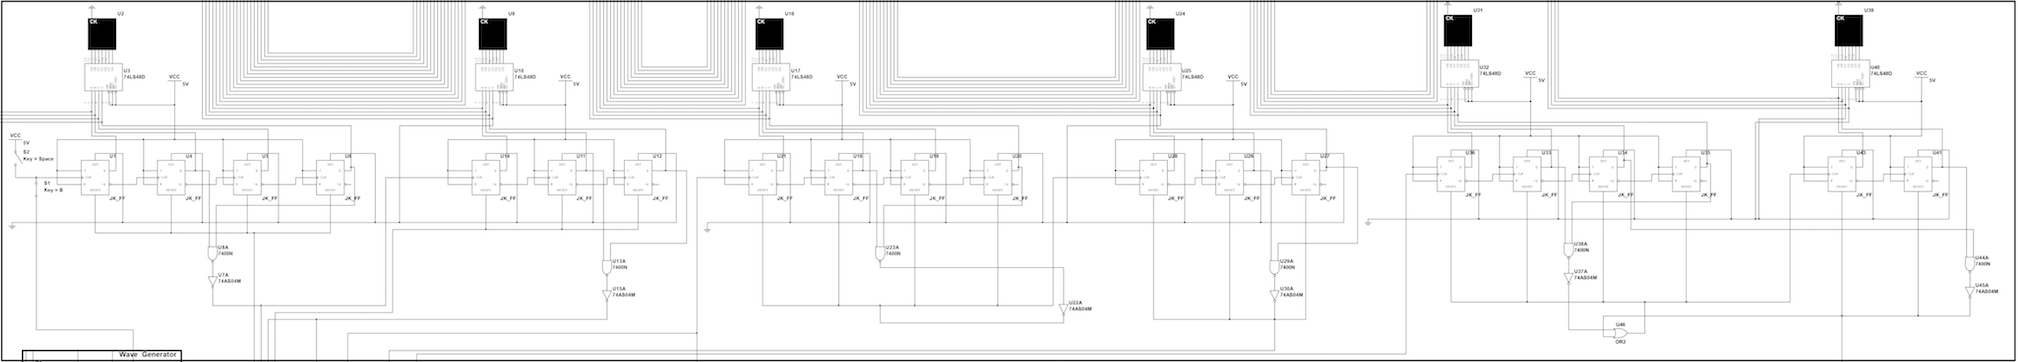
\includegraphics[scale=0.53]{Basic.png}


\subsection{Time Adjust Part}
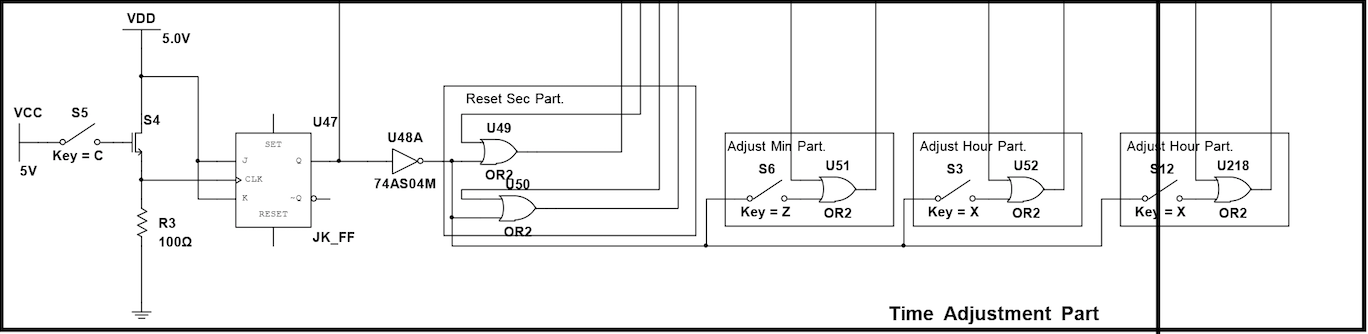
\includegraphics[scale=0.70]{Time.png}

\subsection{Show-Day Part}
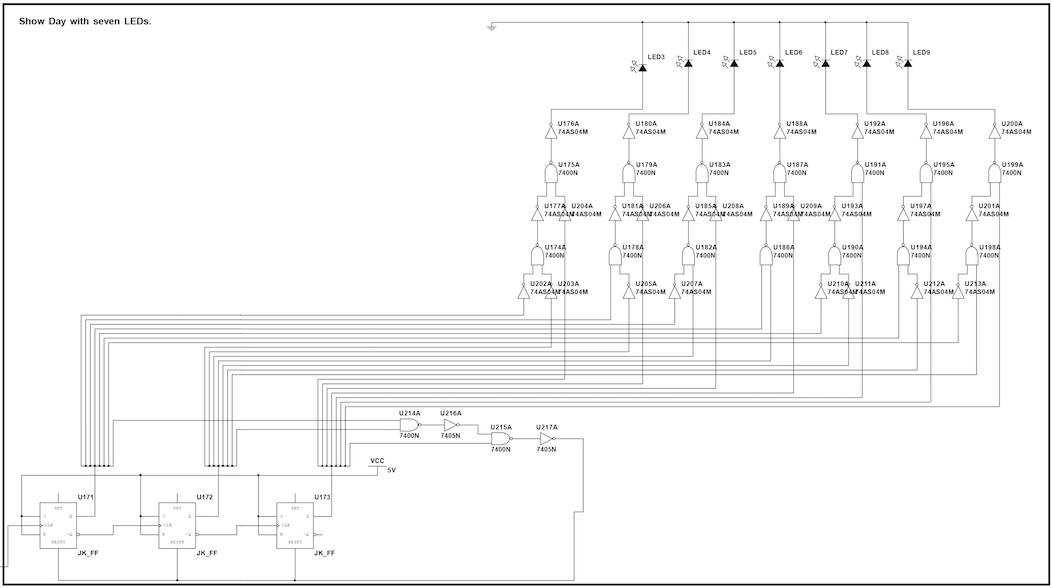
\includegraphics[scale=0.90]{Day.png}
\frameboxbegin{Tips}
Using 7 Led Lights to indicate From Mon. to Sun.
\frameboxend

\subsection{Alarm Part}
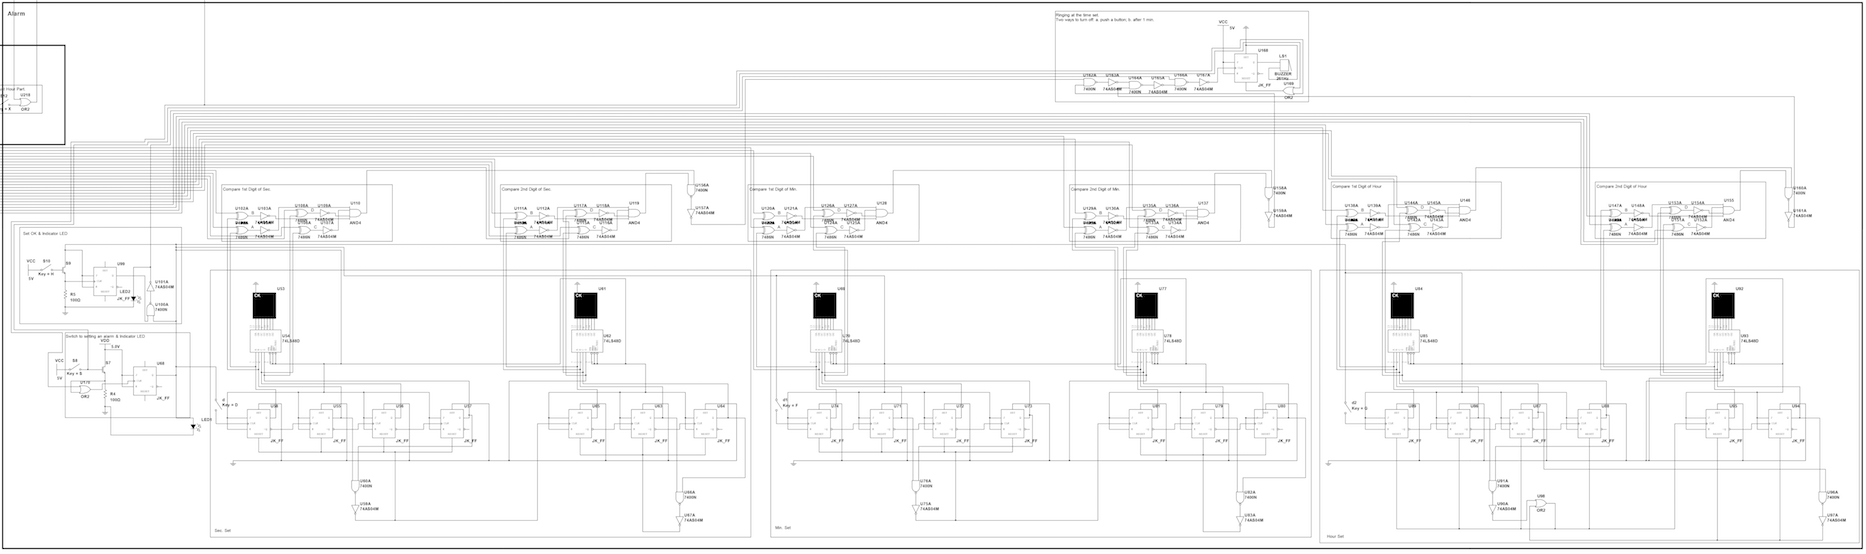
\includegraphics[scale=0.55]{Alarm.png}

\clearpage

\section{Schematic Diagram}
\includegraphics[scale=0.18]{Simulation.png}
\end{document}          
